\documentclass{article}
\usepackage{lib/setup}
\usepackage{hyperref}
\addbibresource{mybibliography.bib}


%%%%%%%%%%%%%%%%%%%%%%%%%%%%%%%%%%%%%%%%%%%%%%%%%%%%%%%%%%%%%%%%%%%%%%%%%%%%%%%%
%%%%%%%%%%%%%%%%%%%%%%%%%%%%%%%%%%%%%%%%%%%%%%%%%%%%%%%%%%%%%%%%%%%%%%%%%%%%%%%%
%%%%%%%%%%%%%%%%%%%%%%%%%%%%%%%%%%%%%%%%%%%%%%%%%%%%%%%%%%%%%%%%%%%%%%%%%%%%%%%%
% Set up your information
%%%%%%%%%%%%%%%%%%%%%%%%%%%%%%%%%%%%%%%%%%%%%%%%%%%%%%%%%%%%%%%%%%%%%%%%%%%%%%%%
\subtitle{Component implementation and testing}
\title{The Shell CPU}
\author{Jonathan Rice Shelley II}
\date{\today}
\headerTitle{Shell CPU}
\subject{Version 1.0}

%%%%%%%%%%%%%%%%%%%%%%%%%%%%%%%%%%%%%%%%%%%%%%%%%%%%%%%%%%%%%%%%%%%%%%%%%%%%%%%%
%%%%%%%%%%%%%%%%%%%%%%%%%%%%%%%%%%%%%%%%%%%%%%%%%%%%%%%%%%%%%%%%%%%%%%%%%%%%%%%%
%%%%%%%%%%%%%%%%%%%%%%%%%%%%%%%%%%%%%%%%%%%%%%%%%%%%%%%%%%%%%%%%%%%%%%%%%%%%%%%%

\newcommand{\stitle}{HDL and Verification}

% BEGIN DOCUMENT
\begin{document}
\maketitle

\section{Contents}
\begin{par}
	\begin{enumerate}
	\item \nameref{overview}
	\item \nameref{CTRL_TEST}
	\item \nameref{compd}
	\end{enumerate}
\end{par}

\section{Component Implementation and Testing Overview }
\label{overview}
\begin{par}
	This document details the implementation and testing of each unique component in the Shell CPU. The VHDL for each module is to long to be listed in this document and can be found here \href{http:\\google.com}{link}. 
\end{par}

\newpage

\section{Control Unit Verification}
\label{CTRL_TEST}
\begin{par}

	\begin{figure}[H]
		\centering
		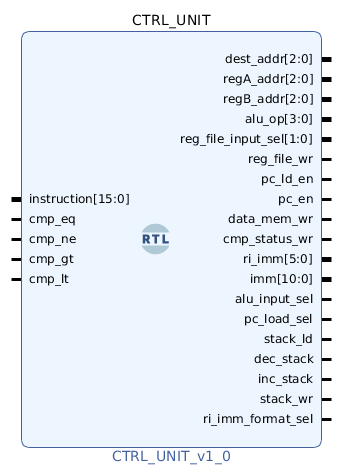
\includegraphics[width=1.5in]{img/ctrl_unit.png}
		\caption{CPU Control Unit}
	\end{figure}

	The control unit is tested against all 23 instructions in the Shell ISA. The order of the instructions tested can be seen in the table below. The control unit output to the instructions is shown in Figure \ref{fig:cpuCtrlTB}.
	
	\begin{center}
		\begin{tabular}{|c|}
			\hline
			\textbf{Instruction test order} \\
			\hline
			hlt \\
			\hline
			add     r1, r2, r3 \\
			\hline
			sub     r1, r2, r3 \\
			\hline
			and     r2, r2, r3 \\
			\hline
			or      r1, r2, r3 \\
			\hline
			xor     r1, r2, r3 \\
			\hline
			nand    r1, r2, r3 \\
			\hline
			lw      r1, r2 \\
			\hline
			sw      r1, r2 \\
			\hline
			asr     r1, r2 \\
			\hline
			asl     r1, r2 \\
			\hline
			cmp     r1, r2 \\
			\hline
			jalr    r1, r2 \\
			\hline
			push    r1 \\
			\hline
			pop r1 \\
			\hline
			lsp r1 \\
			\hline
			addi    r1, 5 \\
			\hline
			subi    r1, 5 \\
			\hline
			lui     r1, 5 \\
			\hline
			beq     5 \\
			\hline
			bne     5 \\
			\hline
			bgt     5 \\
			\hline
			blt     5 \\
			\hline
		\end{tabular}
	\end{center}
	

	\begin{figure}[H]
		\centering
		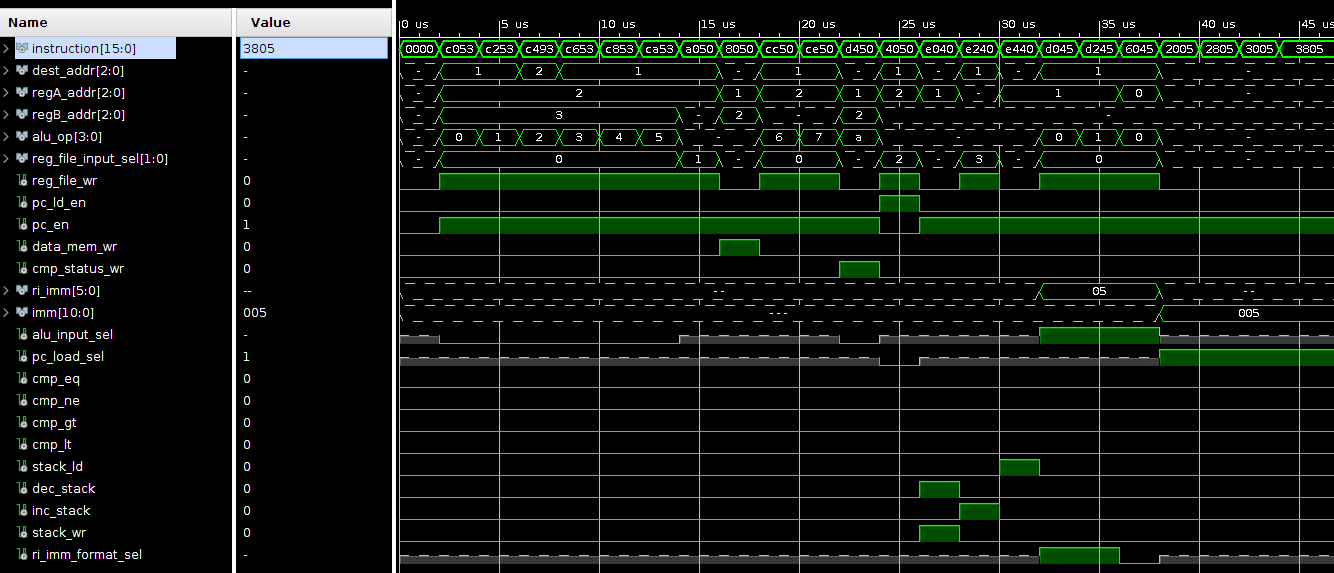
\includegraphics[width=7in]{img/CtrlUnitTB.png}
		\caption{CPU Control Testbench}
		\label{fig:cpuCtrlTB}
	\end{figure}
	
\end{par}

\newpage

\section{Component Testing}
\label{compd}
\begin{par}
	
	\subsection{Arithmetic Logic Unit}
	
	\begin{figure}[H]
		\centering
		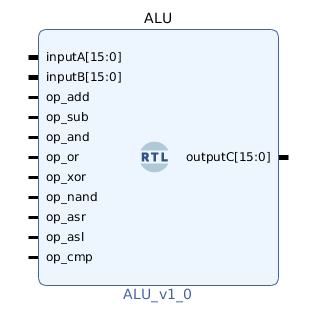
\includegraphics[width=2in]{img/alu.png}
		\caption{Arithmetic Logic Unit}
	\end{figure}

	\textbf{\stitle}
	\begin{par}
		The arithmetic logic unit or ALU performs arithmetic operations on data in the CPU. The block is entirely combinational logic and controlled by its "op" signals. A testbench is created to verify the functionality of the ALU. Figure \ref{fig:alutbfig} shows the ALU undertest performing each operation. 
	\end{par}

	\begin{figure}[H]
		\centering
		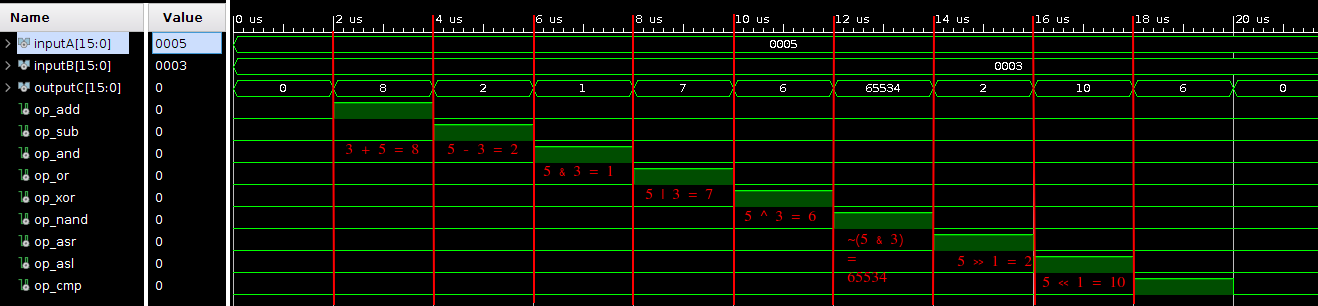
\includegraphics[width=7in]{img/alu_tb.png}
		\caption{Arithmetic Logic Unit}
		\label{fig:alutbfig}
	\end{figure}

	\newpage

	\subsection{Simple Adder}
	
	\begin{figure}[H]
		\centering
		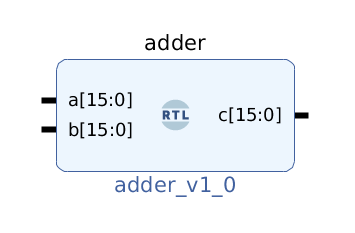
\includegraphics[width=2in]{img/simpleAddr.png}
		\caption{Simple Adder Unit}
	\end{figure}
	
	\textbf{\stitle}
	\begin{par}
		The simple adder block is used to sum values together within the CPU datapath. The block is used once to calculate PC + 1. The block is used a second time to find pc + imm for B-Type instructions. The testbench results for the simple adder can be seen in Figure \ref{fig:addrfig}. From the testbench it can be concluded that the simple adder properly adds the two decimal numbers. 
	\end{par}
	
	\begin{figure}[H]
		\centering
		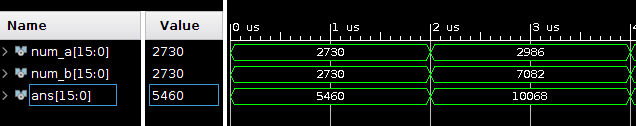
\includegraphics[width=7in]{img/simpleAddrTB.png}
		\caption{Simple Adder Unit Testbench}
		\label{fig:addrfig}
	\end{figure}

	\newpage

	\subsection{Arithmetic Logic Unit Controller}
	
	\begin{figure}[H]
		\centering
		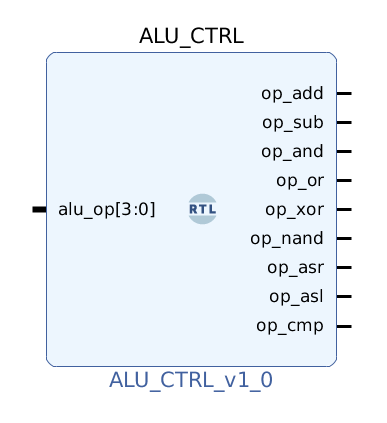
\includegraphics[width=2in]{img/aluCtrl.png}
		\caption{Arithmetic Logic Unit Controller}
	\end{figure}

	\textbf{\stitle}
	\begin{par}
		The arithmetic logic unit controller is used to interpret the ALU op codes from the CPU controller. The outputs of the arithmetic logic unit controller directly control what operation the ALU performs. The ALU control unit can be seen correctly decoding alu\_op in Figure \ref{fig:aluCtrlfig}.
	\end{par}


	\begin{figure}[H]
		\centering
		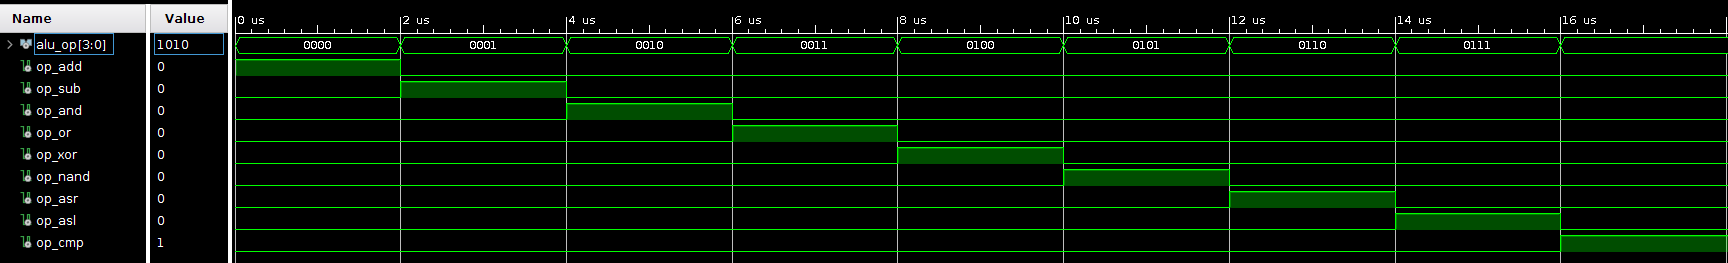
\includegraphics[width=7in]{img/alu_ctrl_tb.png}
		\caption{Arithmetic Logic Unit Controller Testbench Results}
		\label{fig:aluCtrlfig}
	\end{figure}

	\newpage
	
	\subsection{Two to One Multiplexer}
	
	\begin{figure}[H]
		\centering
		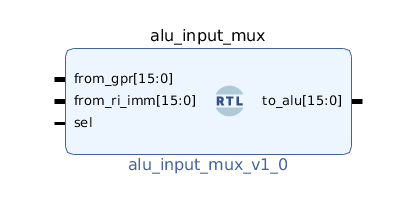
\includegraphics[width=1.5in]{img/aluMux.png}
		\caption{Two to One Multiplexer}
	\end{figure}
	
	\textbf{\stitle}
	\begin{par}
		The two to one multiplexer is used throughout the datapath to mux 16-bit buses. The functionality of the mux is verified as seen in Figure \ref{fig:muxtb}.
	\end{par}


	\begin{figure}[H]
		\centering
		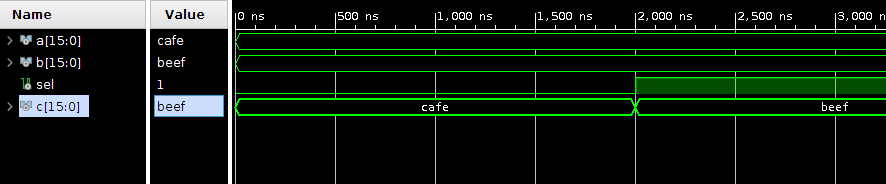
\includegraphics[width=7in]{img/2to1muxtb.png}
		\caption{Two to One Multiplexer Testbench}
		\label{fig:muxtb}
	\end{figure}
	
	\newpage
	
	\subsection{Comparator Status Register}
	
	\begin{figure}[H]
		\centering
		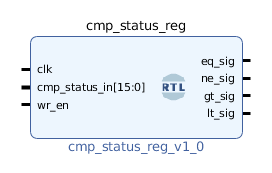
\includegraphics[width=1.5in]{img/cmpStat.png}
		\caption{Comparator Status Register}
	\end{figure}
	
	\textbf{\stitle}
	\begin{par}
		The comparator status register stores the results of a comparison. The testbench for this component can be seen in Figure \ref{fig:cmpregtb}.
	\end{par}

	\begin{figure}[H]
		\centering
		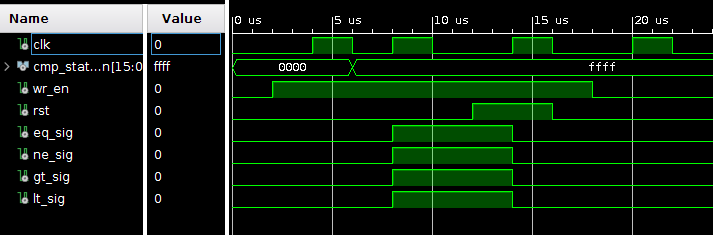
\includegraphics[width=5in]{img/cmpregtb.png}
		\caption{Comparator Status Register Testbench}
		\label{fig:cmpregtb}
	\end{figure}

	\newpage
	
	\subsection{11-bit Immediate Sign Extend}
	
	\begin{figure}[H]
		\centering
		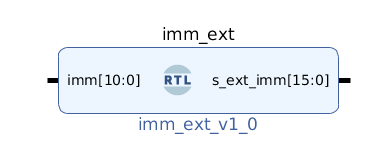
\includegraphics[width=2in]{img/immExt.png}
		\caption{11-bit Immediate Sign Extend}
	\end{figure}
	
	\textbf{\stitle}
	\begin{par}
		Used to sign extend 11-bit immediates from B-type instructions. Verification of this component can be seen in Figure \ref{fig:immExtTb}.
	\end{par}

	\begin{figure}[H]
		\centering
		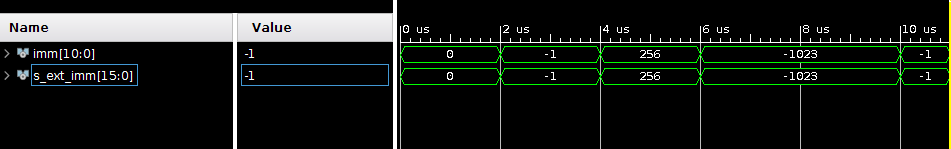
\includegraphics[width=5in]{img/immExtTB.png}
		\caption{11-bit Immediate Sign Extend Testbench}
		\label{fig:immExtTb}
	\end{figure}
	
	\newpage
	
	\subsection{Program Counter Register}
	
	\begin{figure}[H]
		\centering
		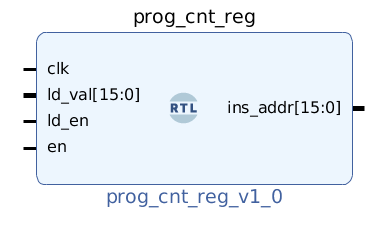
\includegraphics[width=2in]{img/progCnt.png}
		\caption{Program Counter Register}
	\end{figure}
	
	\textbf{\stitle}
	\begin{par}
		Program counter used to keep the address of the next instruction in memory. Verification of the program counter can be seen in Figure \ref{fig:progcnttb}.
	\end{par}
	
	\begin{figure}[H]
		\centering
		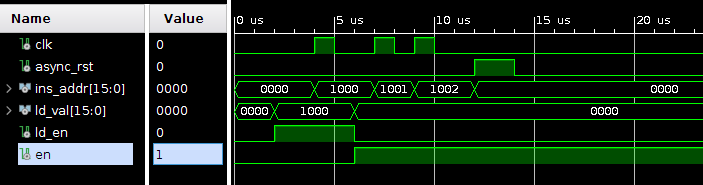
\includegraphics[width=6in]{img/progCntTB.png}
		\caption{Program Counter Register Testbench}
		\label{fig:progcnttb}
	\end{figure}

	\newpage

	\subsection{General Purpose Register File}
	
	\begin{figure}[H]
		\centering
		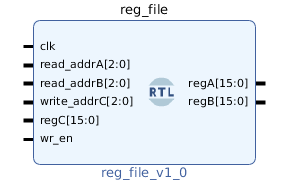
\includegraphics[width=1.6in]{img/regFile.png}
		\caption{General Purpose Register File}
	\end{figure}
	
	\textbf{\stitle}
	\begin{par}
		GPR (General Purpose Register) file is used to store temporary values during computation. The verification of the register file can be seen in Figure \ref{fig:gprtb}.
	\end{par} 

	\begin{figure}[H]
		\centering
		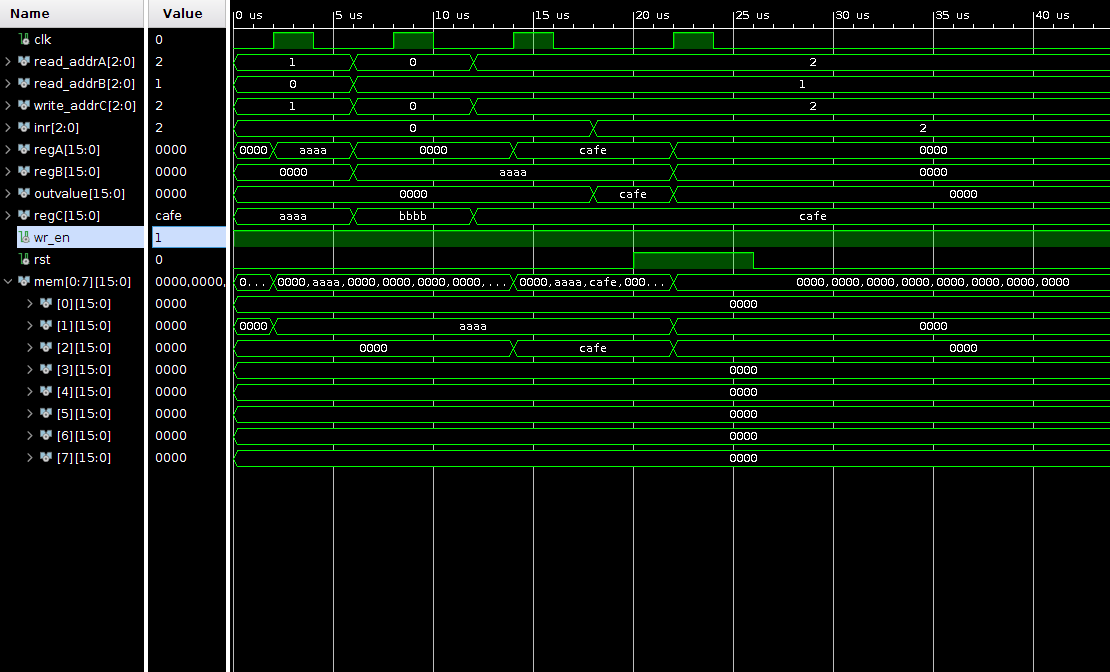
\includegraphics[width=6in]{img/regFileTB.png}
		\caption{General Purpose Register File}
		\label{fig:gprtb}
	\end{figure}

	\newpage
	
	\subsection{Register File Input Multiplexer}
	
	\begin{figure}[H]
		\centering
		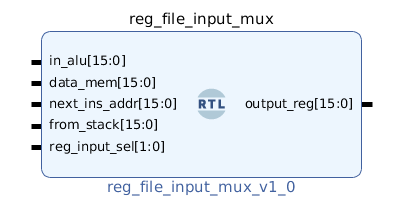
\includegraphics[width=2in]{img/regFileMux.png}
		\caption{Register File Input Multiplexer}
	\end{figure}
	
	\textbf{\stitle}
	\begin{par}
		Used to multiplex the data input to the GPR file. The verification of this component can be seen in Figure \ref{fig:gprMuxTB}.
	\end{par}
	
	\begin{figure}[H]
		\centering
		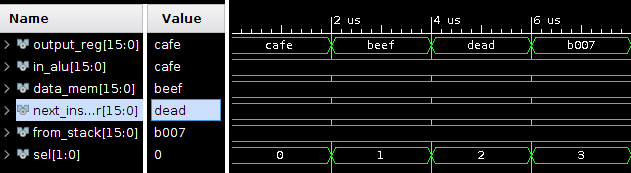
\includegraphics[width=5in]{img/regFileMuxTB.png}
		\caption{Register File Input Multiplexer}
		\label{fig:gprMuxTB}
	\end{figure}
	
	\newpage

	\subsection{RI-Type Zero Extend Immediate \& RI-Type Immediate Upper 6-bit Concatenation}
	
	\begin{figure}[H]
		\centering
		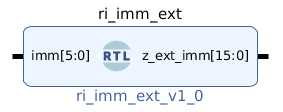
\includegraphics[width=2in]{img/riImmExt.png}
		\caption{RI-Type Zero Extend Immediate}
	\end{figure}

	\begin{figure}[H]
		\centering
		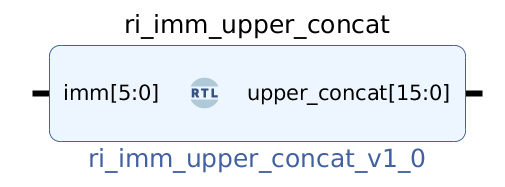
\includegraphics[width=2in]{img/upcon.png}
		\caption{RI-Type Immediate Upper 6-bit Concatenation}
	\end{figure}
	
	\textbf{\stitle}
	\begin{par}
		The immediate zero extend module and immediate upper 6-bit concatenation module are verified below in Figure \ref{fig:ri_imm_tb}. 
	\end{par}

	\begin{figure}[H]
		\centering
		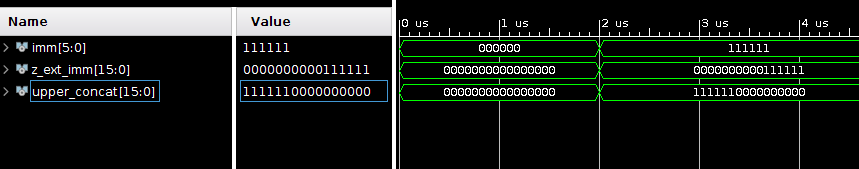
\includegraphics[width=7in]{img/riExtTB.png}
		\caption{RI-Type Zero Extend Immediate}
		\label{fig:ri_imm_tb}
	\end{figure}

	\newpage
	
	\subsection{Stack Pointer Register}
	
	\begin{figure}[H]
		\centering
		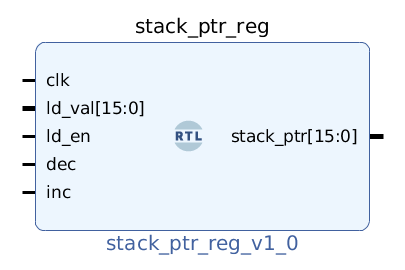
\includegraphics[width=2in]{img/stackPtr.png}
		\caption{Stack Pointer Register}
	\end{figure}

	\textbf{\stitle}
	\begin{par}
		Stack pointer register maintains stack pointer. Verification of the stack pointer module can be seen in Figure \ref{fig:stackPtrTB}.
	\end{par}

	\begin{figure}[H]
		\centering
		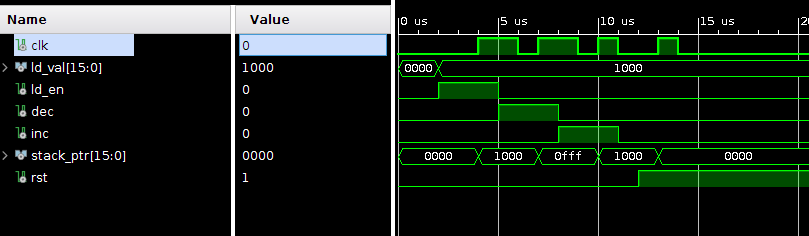
\includegraphics[width=7in]{img/stackPtrTB.png}
		\caption{Stack Pointer Register}
		\label{fig:stackPtrTB}
	\end{figure}

\end{par}

\newpage




\end{document}